\documentclass[11pt,a4paper]{article}
\usepackage[T1]{fontenc}
\usepackage{lmodern,amsmath,amssymb,amsthm,mathtools}
\DeclareMathAlphabet{\mathsf}{OT1}{lmr}{m}{n}
\usepackage[margin=25mm,headheight=15pt]{geometry}
\usepackage{graphicx,booktabs,array,tabularx,longtable}
\usepackage[dvipsnames]{xcolor}
\usepackage{microtype,enumitem,fancyhdr,needspace}
\usepackage[colorlinks=true,linkcolor=MidnightBlue,citecolor=MidnightBlue,urlcolor=MidnightBlue]{hyperref}
\usepackage{bookmark}
\hypersetup{pdftitle={Spatial Observation and Causal Transport with Storage in the Reciprocal Chiral Exchange Candidate},pdfauthor={Hilmir Frímann Halldórsson (pzychozen)},pdfsubject={Research edition v0.1 — project-internal review complete; author-authorized for repository publication.},pdfkeywords={C6 observation, causal transport, positive storage, reciprocal exchange, 10 November 2026}}
\setlength{\parindent}{0pt}\setlength{\parskip}{4pt}\setlength{\emergencystretch}{3em}
\setlist{nosep,leftmargin=*}\numberwithin{equation}{section}
\theoremstyle{definition}\newtheorem{theorem}{Theorem}[section]
\newtheorem{proposition}[theorem]{Proposition}
\newtheorem{lemma}[theorem]{Lemma}
\newtheorem{corollary}[theorem]{Corollary}
\theoremstyle{definition}\newtheorem{definition}[theorem]{Definition}
\theoremstyle{remark}\newtheorem{remark}[theorem]{Remark}
\newcommand{\R}{\mathbb R}\newcommand{\CC}{\mathbb C}
\newcommand{\norm}[1]{\left\lVert#1\right\rVert}\newcommand{\abs}[1]{\left|#1\right|}
\newcommand{\ip}[2]{\left\langle#1,#2\right\rangle}
\newcommand{\dd}{\,\mathrm d}\newcommand{\Bcal}{\mathcal B}\newcommand{\KG}{\mathcal K_G}
\newcommand{\KGz}{\mathcal K_{G,0}}\newcommand{\FF}{\mathcal F}\newcommand{\Dcal}{\mathcal D}
\newcommand{\Wcal}{\mathcal W}\newcommand{\Hcal}{\mathcal H}\newcommand{\Ycal}{\mathcal Y}
\newcommand{\ccar}{c_{\rm car}}\newcommand{\Fn}{F_{\rm native}}\newcommand{\Gmat}{\mathbf G}
\newcommand{\Rb}{R_{\rm ball}}\newcommand{\RG}{R_\Gamma}\newcommand{\ii}{\mathbf1}
\newcommand{\sourcepath}[1]{\texttt{\detokenize{#1}}}
\pagestyle{fancy}\fancyhf{}\fancyhead[L]{\small Spatial observation and causal transport}\fancyhead[R]{\small v0.1}\fancyfoot[C]{\thepage}
\begin{document}
\hypersetup{pageanchor=false}
\begin{titlepage}\centering
\vspace*{10mm}
{\LARGE\bfseries Spatial Observation and Causal\\[3mm]Transport with Storage in the\\[3mm]Reciprocal Chiral Exchange Candidate\par}
\vspace{10mm}
{\large Hilmir Frímann Halldórsson (pzychozen)\par}\vspace{4mm}
{10 November 2026\par}\vspace{5mm}
{\small Research edition v0.1\par Project-internal review complete; author-authorized for repository publication\par}
\vspace{9mm}
\begin{minipage}{0.94\textwidth}
\textbf{Abstract.}
The inherited C6 formula observes a periodic carrier at six central broken boundaries through retarded, distance-weighted histories. We establish its bounded causal action on a complete space-time history domain, distinguish that estimate from point records, and derive its finite-window temporal adjoint. On sufficiently long windows the forward part of that adjoint is advanced; a formal negative-adjoint force leaves a signed prehistory term in the work account. We then declare one stateful causal extension of the reciprocal chiral exchange candidate. Two traveling fields on static delay intervals and a separate receiving field have nonnegative quadratic stocks. Spatial effort/flow coupling yields exact matched work without requiring the mixing operator to be contractive. A method-of-steps argument proves unique global forward mild evolution for every finite-energy preparation, with locally square-integrable boundary signals and exact augmented exchange conservation. C6 remains the direct component of the loaded receiving equation, whose return, loading and arbitrary-profile startup terms are retained explicitly. The original native map retains its finite-window baseline accounting formula. Empty added states impose positive receiving and return delays; a constant carrier preload produces strict receiving and a nonzero incoming return on specified short intervals. This witness is carrier-funded and does not establish native recovery. The result is a mathematical transport/storage connection; its physical curved-route, material and clock correspondence remains open.
\end{minipage}
\vfill
\begin{minipage}{0.94\textwidth}\small
\textbf{Preparation and status.} Hilmir Frímann Halldórsson provides authorship and geometric direction. GPT contributed formulation and project-internal mathematical review; Codex performed independent verification and manuscript preparation. W01--W05 and T01--T07 are accepted at their stated hypotheses, with documentary clarification D01. The author has authorized repository publication of this internally reviewed research edition. No external peer review or formal machine verification is claimed.
\end{minipage}
\end{titlepage}
\hypersetup{pageanchor=true}\setcounter{page}{2}
\setcounter{tocdepth}{1}\tableofcontents
\vspace{7mm}
\textbf{Reading guide.} Sections~\ref{sec:observation}--\ref{sec:conditional} explain what a delayed observation and its temporal dual do establish. Sections~\ref{sec:transport}--\ref{sec:evolution} declare and analyze a different, stateful connection. Sections~\ref{sec:preparation}--\ref{sec:activity} identify its exact observation, preparation and activity scope. The physical correspondence is discussed in Section~\ref{sec:discussion}; appendices record notation and accepted-claim coverage.
\clearpage
\section{Question and progression of the argument}\label{sec:question}
The reciprocal chiral exchange candidate couples a finite native state to a periodic carrier and an unplaced reversible receiver through finite distributed profiles. Its exact work account establishes actual changes of trial stocks. The preceding central-route and six-opening correspondence study showed why those changes alone do not identify completed spatial travel: receiving can precede selected carrier activity, and the retained carrier is separated from all six central broken boundaries and their individual convex enclosures at the common registration~\cite{centralpaper}. That separation is compatible with observing the carrier from the boundaries. It does not supply a load there, and it does not assign zero to an undefined physical aperture flux.

The inherited C6 formula provides a definite retarded observation. It integrates two carrier components, encoded as a scalar and a tangent vector, with endpoint-distance delay and inverse-distance weight. The first question is what that formula defines on the actual central arcs and what its exact mathematical dual says about work. The second is constructive: can a declared extension retain that observation as a direct component while supplying causal evolution, nonnegative intermediate storage and matched work?

We answer these questions in one progression. First, the actual geometry supplies finite measures and a complete history horizon. A space-time estimate gives a bounded causal observation operator; a different, stronger regularity hypothesis supplies continuous point records. The finite-window temporal adjoint necessarily includes prehistory and, on sufficiently long windows, depends on future test values. Its direct use as a formal carrier force therefore provides neither a causal load nor an instantaneous power identity. The associated integrated work identity retains a signed prehistory pairing.

Next we declare two traveling states on a continuum of static delay intervals and a separate receiving field indexed by the central arcs. An isometric duplication and a bounded spatial mixer factor C6 exactly. The mixer and its same-time adjoint enter effort/flow boundary relations; they are not the temporal adjoint of the retarded operator. Characteristics supply time traces and a nonnegative transport stock. A local input-energy estimate, obtained before assuming total conservation, continues the coupled solution through each delay slab. This proves global forward mild evolution and exact augmented exchange conservation for every finite-energy preparation. Finally, the full receiving equation retains C6, return, loading and startup contributions; the original native jumps retain their baseline account; and a specified carrier preload gives strict delayed receiving and an incoming-return witness.

The mathematical foundations are the accepted project-internal investigations W01--W05 and T01--T07~\cite{Wreview,Treview}. The present paper provides their principal derivations rather than treating the acceptance records or their exact-algebra counts as proofs. The two investigations have different roles: W analyzes the inherited observation and a conditional work pairing, whereas T declares additional states, metrics and boundary laws and proves their properties. The construction is one modeling choice, not a unique deduction from C6.

Wave-variable and passivity-based treatment of delayed interactions is established methodology~\cite{niemeyer}. That reference supplies context for the general method, not a black-box theorem for this infinite-dimensional system. The particular operators, arbitrary-profile startup terms, nonlinear continuation argument and activity witness are established below. No novelty is claimed for the general use of traveling variables to account for delayed exchange.

\begin{table}[htbp]\centering\small
\begin{tabularx}{\textwidth}{@{}p{.20\textwidth}X@{}}\toprule
Role & Ingredients and conclusions\\\midrule
Inherited & Static carrier/G geometry, C6 delay and weight, original RX native/carrier/old-receiver equations, profiles, trial stocks and native map.\\[3pt]
Declared here & Product state metric, duplicated channels, two traveling fields, new receiving field, coupling strength and near/far boundary relations.\\[3pt]
Proved & Bounded observation, qualified temporal duality, causal mild extension, nonnegative stocks, exact work, finite native-step account and carrier-funded activity.\\[3pt]
Still open & Physical route, material energy density, overlap of channels, interface location, load meaning, speed and clock calibration.\\\bottomrule
\end{tabularx}
\caption{Definitions, modeling choices and proved properties have different status.}\label{tab:roles}
\end{table}

The intended physical picture retains stationary supports, a central meeting region, opposed directions, outward spreading, a curved return and possible transfer elsewhere. Local exchange and a larger circuit are compatible aims. This paper completes an abstract mathematical connection while leaving that physical attachment explicit as subsequent work.

\section{Static geometry and the retained reciprocal exchange}\label{sec:setting}
\subsection{The six actual arcs and the selected carrier}
Use width-one centered coordinates relative to O and a static parameter $0\le\tau_g\le h_g$. Define
\begin{equation}\label{eq:geomconstants}
r_g=\frac{\sqrt3}{6},\quad d_g=1-\frac{\sqrt2}{2},\quad
a_g=\frac{d_g}{2},\quad h_g=\frac{\sqrt2-1}{2},\quad H_0=\frac12=h_g+d_g.
\end{equation}
Let $e_i=(\cos(-\pi/2+i\pi/3),\sin(-\pi/2+i\pi/3))$, with indices modulo six. For the horizontal quarter-turn $J_\perp$, put
\begin{equation}\label{eq:horizmap}
A^\perp_{\tau_g}=I-\frac{\tau_g}{r_g}J_\perp,\qquad
(A^\perp_{\tau_g})^TA^\perp_{\tau_g}=D(\tau_g)^2I,
\quad D(\tau_g)^2=1+\frac{\tau_g^2}{r_g^2}\le D_*^2:=10-6\sqrt2.
\end{equation}
The vertices and actual broken arcs are~\cite{CCgeometry}
\begin{align}
T_i&=(a_ge_i,h_g),&B_i&=(a_gA^\perp_{\tau_g}e_i,-h_g),\notag\\
U_k&=(r_ge_{2k},H_0),&L_k&=(r_gA^\perp_{\tau_g}e_{2k},-H_0),\label{eq:vertices}\\
G_k^+&=[U_k,T_{2k+1}]\cup[T_{2k+1},U_{k+1}],&
G_k^-&=[L_k,B_{2k+1}]\cup[B_{2k+1},L_{k+1}],\label{eq:actualG}
\end{align}
for $k=0,1,2$, with $U_3=U_0$ and $L_3=L_0$. A common width $w>0$ multiplies every centered coordinate before translation by O. MINUS reflects the entire registered construction by $S=\operatorname{diag}(-1,1,1)$ with labels retained. The labels identify arcs, not propagation directions. No tip-to-tip chord, aperture interior, normal or physical surface measure is added.

Let G denote their disjoint labeled union at width w, equipped with ordinary arclength $d\ell_X$. Shared endpoints are null sets for this measure. The selected carrier is the one source circle $\Gamma_0$, not three instantiated carriers. With $u=(0,1,0)$ in PLUS,
\begin{align}
K_c&=\frac{\sqrt3}{12}+\frac{\sqrt6}{4},&
a_c&=\frac{K_c}{1+\sqrt3/2},&\RG&=\frac{\sqrt7}{2}a_c,&L&=2\pi w\RG,\label{eq:circleconstants}\\
\gamma_w(s)&=O+wK_cu+w\RG(\cos\chi\,u+\sin\chi\,e_z),\notag\\
\chi&=\frac{s}{w\RG},\qquad \hat t(s)=-\sin\chi\,u+\cos\chi\,e_z.\label{eq:circle}
\end{align}
Here $s\in S_L:=\R/L\mathbb Z$ is physical arclength and $|\hat t|=1$. The reflected hand applies S to the full geometry. The accepted separation theorem gives the uniform input
\begin{equation}\label{eq:clearance}
d_X(s):=|X-\gamma_w(s)|>\delta_w:=\frac{297}{5000}w
\qquad(X\in G,\ s\in S_L).
\end{equation}
It also covers each arc's individual convex enclosure, but those enclosures are mathematical bounding sets, not adopted apertures~\cite{centralpaper,SOreview}. Its proof is not repeated here.

\begin{proposition}[Geometry and history bounds]\label{prop:geometry}
Put $v_0^2=r_g^2+a_g^2-a_gr_g$ and $\Rb^2=13/12-\sqrt2/2$. Every actual G point lies in the ball $|X-O|\le w\Rb$. The total labeled length is
\begin{align}
M=M_w(\tau_g)&=6w\left[\sqrt{v_0^2+d_g^2}+\sqrt{D(\tau_g)^2v_0^2+d_g^2}\right]\label{eq:Glength}\\
&\le M_{w,*}:=6w\left[\sqrt{v_0^2+d_g^2}+\sqrt{D_*^2v_0^2+d_g^2}\right].\notag
\end{align}
For an independent $c_e>0$, a sufficient history horizon is
\begin{equation}\label{eq:horizon}
\begin{gathered}
\Theta=\frac{w(K_c+\RG+\Rb)}{c_e},\\
0<\theta_-:=\min_{s,X}\frac{d_X(s)}{c_e}
\le\theta_X(s):=\frac{d_X(s)}{c_e}
\le\theta_+:=\max_{s,X}\frac{d_X(s)}{c_e}\le\Theta.
\end{gathered}
\end{equation}
These statements hold for every admitted fixed static parameter and both hands under common scaling.
\end{proposition}
\begin{proof}
Direct expansion gives
\begin{equation}\label{eq:ballmargin}
r_g^2+h_g^2+H_0^2=\Rb^2,\qquad
r_g^2-a_g^2=\frac{6\sqrt2-7}{24}>0,\qquad
\Rb^2-|L_k|^2=h_g^2-\tau_g^2\ge0.
\end{equation}
The strict inequality follows by squaring positive quantities: $72>49$. A lower elbow has smaller squared norm than a lower tip by
$D^2(r_g^2-a_g^2)+(H_0^2-h_g^2)>0$; the upper comparison uses $D=1$. Norm convexity extends the endpoint bound along every segment. The lower-tip bound is attained at $\tau_g=h_g$, but this does not assert attainment of the later distance ceiling.

The underlying adjacent unit directions satisfy $e_i\cdot e_{i+1}=1/2$, including the wraparound pair $e_5,e_0$ for the $T_5$--$U_0$ and $B_5$--$L_0$ edges. The upper horizontal edge has squared length
$v_0^2=(r_g-a_g/2)^2+3a_g^2/4>0$.
There are six upper edges with squared length $v_0^2+d_g^2$ and six lower edges with squared length $D^2v_0^2+d_g^2$. Only horizontal lengths gain D; the vertical difference remains $d_g$. Summing proves~\eqref{eq:Glength}, maximized at $\tau_g=h_g$. At zero it is twelve equal edge lengths. Scaling and full orthogonal reflection preserve these statements.

Finally $|\gamma_w(s)-O|\le w(K_c+\RG)$, so the triangle inequality gives $d_X(s)\le w(K_c+\RG+\Rb)$. Compactness and the accepted strict clearance give the positive attained extrema in~\eqref{eq:horizon}. This ceiling is sufficient, not optimized.
\end{proof}

$\Rb$ is a full three-dimensional ball radius. Cylindrical radius would instead be $\rho_\perp(X)=\sqrt{(X_1-O_1)^2+(X_2-O_2)^2}$; it omits height and is not used for the enclosing-ball argument. Neither radius defines a material wall. The static $\tau_g$ is not a time coordinate.

\subsection{State, profiles and original work metric}
The native state is $\Omega=a_N+ib_N\in\CC^3$, or $x=(a_N,b_N)\in\R^6$, with $I=|x|^2$. The fixed rank-two source matrix K retains the original registration and gain. Define
\begin{equation}\label{eq:drive}
f(x)=K(a_N\times b_N),\quad J_f(x)=D_xf(x),\quad J_f(x)x=2f(x).
\end{equation}
The last identity is differentiation of the degree-two cross product in the direction x. Source orientation signs are already in K; contact labels do not insert new propagation signs.

On the carrier let $Q=(p,r_c)$ and keep the two finite normalized periodic tents,
\begin{equation}\label{eq:profiles}
b_\sigma(s)=\epsilon_c^{-1}\left(1-\frac{|\operatorname{wrap}_L(s-s_\sigma)|}{\epsilon_c}\right)_+,
\quad \sigma\in\{+,-\},\quad 0<\epsilon_c<\eta_{\rm geom}.
\end{equation}
Here $s_\pm=L/2\mp\eta_{\rm geom}$, with
$\eta_{\rm geom}=w\RG\arctan(2/\sqrt3)$, and $\operatorname{wrap}_L$ takes values in $[-L/2,L/2)$. These disjoint profiles belong to periodic H1, have unit integral, and represent arclength width, not tube radius. Define
\begin{equation}\label{eq:ports}
\Bcal v=b_+v_++b_-v_-,\qquad
y=\Bcal^*p=\left(\int b_+p\dd s,\int b_-p\dd s\right)^T.
\end{equation}
All unqualified s integrals cover one full circle. The retained reciprocal equations and stocks are~\cite{RXcandidate,RXpower}
\begin{equation}\label{eq:RX}
\begin{aligned}
q&=\eta_N f(x)-\eta_Rz,&
\dot x&=-\frac{\eta_N}{2\alpha_N}J_f(x)^Ty,&
\dot z&=\frac{\eta_R}{\beta_R}y,\\
p_t+\ccar(r_c)_s&=\Bcal q,&(r_c)_t+\ccar p_s&=0,
\end{aligned}
\end{equation}
\begin{equation}\label{eq:RXstocks}
H_N=\frac{\alpha_N}{2}|x|^2,\quad
H_C=\frac12\int(p^2+r_c^2)\dd s,\quad
H_R=\frac{\beta_R}{2}|z|^2,\quad H_{\rm RX}=H_N+H_C+H_R.
\end{equation}
Here $\alpha_N,\beta_R,\ccar>0$ and $\eta_N,\eta_R\ge0$ are fixed finite allowed parameters. The old receiver $z\in\R^2$ has no assigned G or material location. Its two coordinates are not two additional physical holes. The later field $\zeta$ has a different state and metric.

The tents give bounded maps $\Bcal:\R^2\to H^1_{\rm per}$ and $\Bcal^*:L^2\to\R^2$. The free generator
\begin{equation}\label{eq:freegroup}
A_c(p,r_c)=(-\ccar(r_c)_s,-\ccar p_s),\qquad D(A_c)=H^1_{\rm per}(S_L;\R^2)
\end{equation}
generates a unitary strongly continuous group $S_c(t)$: in $(p\pm r_c)/\sqrt2$ coordinates it translates in opposite directions. This elementary structure, not automatic reuse of the old nonlinear theorem, supports the new existence proof.

\section{Causal observation and its finite-window temporal adjoint}\label{sec:observation}
The geometry now guarantees that the inherited C6 formula can be evaluated away from the carrier. This fact concerns observation, not loading. Set
\begin{equation}\label{eq:spaces}
U=L^2(S_L;\R^2),\qquad Y=L^2(G;\R^4),\qquad
\Hcal_T=L^2([-\Theta,T];U),\qquad \Ycal_T=L^2([0,T];Y),
\end{equation}
where $0<T<\infty$. The measures are $ds\,du$ and $d\ell_X\,dt$, with sums implicit in the labeled G integral. For $a_o=g_o/(4\pi)>0$, let
\begin{equation}\label{eq:As}
A_s(p,r_c)=(p,r_c\hat t(s)),\qquad A_s^*A_s=I_2.
\end{equation}
The ambient C6 observation is~\cite{CCcarrier}
\begin{equation}\label{eq:C6}
(\KG Q)(X,t)=\binom{U_o(X,t)}{V_o(X,t)}
=a_o\int_{S_L}\frac{A_sQ(s,t-\theta_X(s))}{d_X(s)}\dd s.
\end{equation}
Subscripts on $U_o,V_o$ distinguish output components from Hilbert spaces. A fixed orthonormal observation frame E would give $(U_o,E^TV_o)$ instead. E is not the profile operator $\Bcal$. The tangent vector $r_c\hat t$ is not the scalar carrier flux $\ccar p r_c$, and no squared observation norm is declared a receiving store.

\subsection{A history-space bound and its limits}
\begin{theorem}[Bounded causal history observation]\label{thm:observation}
Formula~\eqref{eq:C6}, initially on smooth histories, extends uniquely to a bounded map $\KG:\Hcal_T\to\Ycal_T$, with
\begin{equation}\label{eq:Kbound}
\norm{\KG Q}_{\Ycal_T}\le\frac{a_o\sqrt{LM}}{\delta_w}\norm Q_{\Hcal_T}
\le\frac{a_o\sqrt{LM_{w,*}}}{\delta_w}\norm Q_{\Hcal_T}.
\end{equation}
Its output is defined almost everywhere in space and time and is causal. For histories in $C([-\Theta,T];H^1_{\rm per})$, it has a continuous representative on each labeled arc times $[0,T]$. Evaluation at a single $(X,t)$ is not bounded in the weaker $\Hcal_T$ norm.
\end{theorem}
\begin{proof}
The isometry of $A_s$ and Cauchy--Schwarz in s give
\begin{equation}\label{eq:pointestimate}
|\KG Q(X,t)|^2\le\frac{a_o^2L}{\delta_w^2}
\int_{S_L}|Q(s,t-\theta_X(s))|^2\dd s.
\end{equation}
For fixed s,X substitute $u=t-\theta_X(s)$. The Jacobian is one and
$[-\theta_X(s),T-\theta_X(s)]\subset[-\Theta,T]$. Tonelli and then integration over G give
\begin{equation}\label{eq:translatedestimate}
\int_G\int_0^T\int_{S_L}|Q(s,t-\theta_X(s))|^2\dd s\dd t\dd\ell_X
\le M\norm Q_{\Hcal_T}^2.
\end{equation}
This proves~\eqref{eq:Kbound}. For a difference of representatives that is zero a.e. in $(s,u)$, the same nonnegative triple integral is zero; Fubini makes the s integral independent of representatives for a.e. $(X,t)$. Smooth periodic histories are dense in $\Hcal_T$, giving the unique bounded extension and its agreement with this integral. No single retarded graph through an arbitrary L2 function has been used as an independent trace theorem.

Every input time is earlier than the output time by at least $\delta_w/c_e$. Thus equality of histories through a cutoff implies equality of observations through it, within the stated domains. The estimate needs no extra $\sqrt2$ because $A_s$ is an isometry and no extra $\sqrt T$ because time is already integrated in the history norm. It is an upper bound, not an assertion of an optimal operator norm. Since L and M scale as w while $\delta_w$ scales as w, its displayed uniform constant can be independent of width at fixed gain. The required horizon still scales as $w/c_e$.

For the continuous-record statement, $H^1_{\rm per}\hookrightarrow C^0$ in one dimension is continuous. Time continuity in H1 therefore gives uniform-in-s continuity in time; together with the continuous spatial representatives it gives joint continuity on the compact history domain. Positive clearance and the continuous kernel imply continuity of the integral by dominated convergence, also at arc elbows and endpoints.

To disprove bounded point evaluation, fix $X_0\in G$ and $0<t_0<T$. The smooth periodic graph $u_0(s)=t_0-\theta_{X_0}(s)$ lies strictly inside $[-\Theta,T]$: its lower margin is at least $t_0$, and its upper margin at least $T-t_0+\theta_-$. Choose nonzero smooth periodic $v\ge0$ and $\psi\in C_c^\infty((-1,1))$ with $\psi(0)>0$. For sufficiently small $\varepsilon>0$, put
\begin{equation}\label{eq:narrowgraph}
Q_\varepsilon(s,u)=\left(\varepsilon^{-1/2}v(s)
\psi\!\left(\frac{u-u_0(s)}{\varepsilon}\right),0\right).
\end{equation}
Every bump lies inside the history interval, so direct time substitution gives
$\norm{Q_\varepsilon}_{\Hcal_T}=\norm v_2\norm\psi_2$, independent of $\varepsilon$. But
\begin{equation}\label{eq:pointunbounded}
U_{o,\varepsilon}(X_0,t_0)=a_o\varepsilon^{-1/2}\psi(0)
\int_{S_L}\frac{v(s)}{d_{X_0}(s)}\dd s\longrightarrow+\infty.
\end{equation}
Each history is smooth. This proves unboundedness already on that class and does not contradict continuity under the stronger history topology.
\end{proof}

All required negative-time history must be provided. A carrier value at time zero, even an empty value, does not by itself specify the past needed by C6.

\subsection{The exact temporal adjoint}
For $\lambda=(\lambda_0,\lambda_v)\in\Ycal_T$, extend it by zero outside $[0,T]$, writing $\widetilde\lambda$. The test is mathematical dual data; no physical load units or constitutive interpretation is implicit.

\begin{proposition}[Complete finite-window duality]\label{prop:adjoint}
The Hilbert adjoint $\KG^*:\Ycal_T\to\Hcal_T$ is
\begin{equation}\label{eq:temporaladjoint}
(\KG^*\lambda)(s,u)=a_o\int_G\frac{1}{d_X(s)}
\binom{\widetilde\lambda_0(X,u+\theta_X(s))}
{\hat t(s)\cdot\widetilde\lambda_v(X,u+\theta_X(s))}\dd\ell_X.
\end{equation}
It satisfies
\begin{equation}\label{eq:duality}
\ip{\lambda}{\KG Q}_{\Ycal_T}=\ip{Q}{\KG^*\lambda}_{\Hcal_T},
\qquad\norm{\KG^*}=\norm{\KG},
\end{equation}
and can be supported only in $[-\theta_+,T-\theta_-]\subset[-\Theta,T]$. Its restriction to $u\in[0,T]$ is zero a.e. if $T\le\theta_-$; for $T>\theta_-$ that restriction is, in general, noncausal as an operator on the test history.
\end{proposition}
\begin{proof}
Insert~\eqref{eq:C6} in the left pairing. Its absolute triple integral is bounded by
\[
(a_o/\delta_w)\sqrt{LM}\norm\lambda_{\Ycal_T}\norm Q_{\Hcal_T},
\]
using Cauchy--Schwarz on $(X,t,s)$ and~\eqref{eq:translatedestimate}. Fubini is legitimate. At fixed s,X translate time to $u=t-\theta_X(s)$. The indicator becomes exactly $0\le u+\theta_X(s)\le T$, retained by zero extension, and $A_s^*(\lambda_0,\lambda_v)=(\lambda_0,\hat t\cdot\lambda_v)$. This proves the displayed formula and pairing. No spatial variable changes, so no derivative of the delay or additional Jacobian appears.

Conversely, Cauchy--Schwarz in X bounds the square of~\eqref{eq:temporaladjoint} by
\[
a_o^2M\delta_w^{-2}\int_G|\widetilde\lambda(X,u+\theta_X(s))|^2\dd\ell_X.
\]
Integration in u,s proves the same operator bound and representative independence. The norm equality follows by Hilbert duality; it does not say the bound in~\eqref{eq:Kbound} is sharp. In framed output coordinates the second component must instead contain $\hat t\cdot(E\widetilde\lambda_v)$.

The translated indicator gives the support claim. For $T\le\theta_-$ it vanishes at every u>0; a possible equality at u=0 is a null time endpoint. The full adjoint can still be nonzero on prehistory.

For $T>\theta_-$, choose a carrier point $s_*$ and a point $X_*$ in a segment interior with $\theta_*:=\theta_{X_*}(s_*)<T$. If a minimizer is a tip or elbow, continuity permits moving into a neighboring interior while preserving this strict inequality. Choose $0<u_*<T-\theta_*$ and
\begin{equation}\label{eq:futureepsilon}
0<\varepsilon<\min\{u_*/4,\theta_*/8,(T-u_*-\theta_*)/4\}.
\end{equation}
Shrink circle/arc neighborhoods until $|\theta_X(s)-\theta_*|<\varepsilon$. Take a nonnegative scalar test with a spatial bump positive on a smaller arc patch and a time bump positive for
$|t-(u_*+\theta_*)|<2\varepsilon$, supported where that difference is less than $3\varepsilon$; set $\lambda_v=0$. Its entire support is later than $u_*$ and inside the window. For s in the smaller circle neighborhood and $u\in(u_*-\varepsilon,u_*)$, the shifted time lies in the positive part. Positivity of $a_o/d_X(s)$ makes the scalar adjoint strictly positive on this set of positive $ds\,du$ measure. The test and zero test agree through $u_*$ but their adjoints differ before it. This is noncausal dependence in L2, not an isolated point-value assertion.
\end{proof}

This is a limitation of using this particular temporal adjoint directly as forward feedback. It does not exclude causal systems with extra memory, propagation, storage or different ports. Integrated duality is not instantaneous physical power matching.

\subsection{What present carrier data cannot determine}
\begin{proposition}[An unrestricted-history witness]\label{prop:presenthistory}
On the smooth history domain of C6, the present carrier value alone does not determine its observation.
\end{proposition}
\begin{proof}
Fix an interior arc point $X_0$, $0<t_0<T$, and any $s_0$. The delayed time
$u_*=t_0-\theta_{X_0}(s_0)$ belongs to $(-\Theta,t_0)$. Choose
$0<\varepsilon<\frac12\min\{u_*+\Theta,t_0-u_*\}$ and a nonnegative smooth bump $\phi$ supported in $(u_*-\varepsilon,u_*+\varepsilon)$ with $\phi(u_*)>0$. For example use $\exp[-1/(1-((u-u_*)/\varepsilon)^2)]$ inside that interval and zero outside. The two histories $Q_0=0$ and $Q_1(s,u)=(\phi(u),0)$ are smooth and periodic and have identical zero carrier values at $t_0$. Delay continuity makes $\phi(t_0-\theta_{X_0}(s))>0$ on a circle neighborhood of $s_0$, so
\begin{equation}\label{eq:historywitness}
U_{o,1}(X_0,t_0)=a_o\int_{S_L}\frac{\phi(t_0-\theta_{X_0}(s))}{d_{X_0}(s)}\dd s>0=U_{o,0}(X_0,t_0).
\end{equation}
Continuous records give a difference on a nonempty observation neighborhood too.
\end{proof}

These are arbitrary histories, not two solutions of RX or C1. The proposition establishes no failure of reconstruction from a full $(x,Q,z)$ state, no native-map noninvertibility result and no universal obstruction under a prescribed launch/prehistory protocol. The separate accepted common-phase information result concerns an outlet rule that actually distinguishes common-phase-related native states while exchange outputs agree; it is not strengthened by this witness~\cite{centralpaper,Wreview}.

\section{Conditional added work and the signed prehistory residual}\label{sec:conditional}
Before declaring new dynamics, it is useful to identify exactly what an added-force account would require. Keep the native and old-z equations in~\eqref{eq:RX}, but write a possible carrier force $\FF=(F_p,F_r)$ as
\begin{equation}\label{eq:conditionalforce}
p_t+\ccar(r_c)_s=\Bcal q+F_p,\qquad (r_c)_t+\ccar p_s=F_r.
\end{equation}
This notation alone supplies no force law or existence theorem.

\begin{proposition}[Conditional regional and global work]\label{prop:conditionalwork}
Suppose a solution has sufficient regularity, for example $Q\in C_tH^1_{\rm per}\cap C_t^1L^2$ on each exchange interval, with the retained finite-dimensional equations and integrable added work. Then, distributionally locally and in integrated time globally,
\begin{align}
\partial_t e+\partial_s j&=p\Bcal q+pF_p+r_cF_r,
&e&=\frac{p^2+r_c^2}{2},&j&=\ccar p r_c,\label{eq:localadded}\\
\dot H_{\rm RX}&=P_{\rm add},&P_{\rm add}&=\int_{S_L}(pF_p+r_cF_r)\dd s.\label{eq:addedpower}
\end{align}
With only the original finite native jumps and post-jump endpoints on $[0,T]$,
\begin{equation}\label{eq:conditionalhybrid}
\Delta H_{\rm RX}-B_N=\int_0^T P_{\rm add}(t)\dd t,\qquad
B_N=\sum_{0<t_j\le T}\frac{\alpha_N}{2}
\left[I(\Fn\Omega(t_j^-))-I(\Omega(t_j^-))\right].
\end{equation}
\end{proposition}
\begin{proof}
Multiply~\eqref{eq:conditionalforce} by p and $r_c$ and add. The H1 product rule gives~\eqref{eq:localadded}; periodic integration removes its flux derivative. The carrier source contributes $\eta_N f\cdot y-\eta_Rz\cdot y$ by profile adjointness. Equation~\eqref{eq:drive} and the factor one-half in native feedback give $\dot H_N=-\eta_Nf\cdot y$, while $\dot H_R=\eta_Rz\cdot y$. These cancel the old carrier source, leaving both added terms with plus signs. Between jumps integrate this identity and telescope. Only x jumps, so the finite sum is exactly~\eqref{eq:conditionalhybrid}. The jump at zero is already reflected in the initial post-jump value; one at T is included. No impulsive port work is inserted. The original map is reproduced in Section~\ref{sec:native}.
\end{proof}

Define mathematical test work and a prehistory pairing by
\begin{equation}\label{eq:testpre}
W^{\rm test}=\ip{\lambda}{\KG Q}_{\Ycal_T},\qquad
W_{\rm pre}=\int_{-\Theta}^0\int_{S_L}Q(s,u)\cdot(\KG^*\lambda)(s,u)\dd s\dd u.
\end{equation}
Both are finite on the declared spaces. Calling the former physical receiving work would require dual units and a constitutive meaning for $\lambda$, absent from C6.

\begin{corollary}[Formal negative-adjoint residual]\label{cor:prehistory}
Conditional on a solution covered by Proposition~\ref{prop:conditionalwork} with $\FF=-\KG^*\lambda$ on forward times,
\begin{equation}\label{eq:prehistorybalance}
\boxed{\Delta H_{\rm RX}+W^{\rm test}-B_N=W_{\rm pre}.}
\end{equation}
The right-hand pairing is signed despite its positive coefficient. Zero prehistory is sufficient, not necessary, for it to vanish.
\end{corollary}
\begin{proof}
Split~\eqref{eq:duality} at u=0. Its forward part equals $-\int_0^T P_{\rm add}\dd t$, leaving
$W^{\rm test}=W_{\rm pre}-\int_0^T P_{\rm add}\dd t$.
Substitute~\eqref{eq:conditionalhybrid}. Nonzero prehistory can have zero pairing by disjoint support, orthogonality or signed cancellation; zero prehistory is only one sufficient condition.
\end{proof}

The short-window case is exact: if $T\le\theta_-$, the forward adjoint force is zero a.e., so $\Delta H_{\rm RX}=B_N$ and $W^{\rm test}=W_{\rm pre}$ can still be nonzero. If prehistory is also zero, the short-window observation vanishes a.e. A simple-delay example in Appendix~\ref{app:example} makes the sign and cancellation concrete; it is not the proof for geometry-dependent delays.

Even when $W_{\rm pre}=0$, this is integrated duality, not a causal loading theorem. The formal adjoint force can retain advanced dependence and need not have the stronger regularity assumed for the conditional solution. If a later model declares receiving power $P_G$ and a transit stock $E_{\rm tr}$, a necessary closed balance would be $\dot E_{\rm tr}=-P_{\rm add}-P_G$. Defining a quantity by that residual alone proves neither its nonnegativity, its dynamics nor its material location. The next section instead supplies an explicit state evolution and derives its stock balance.

\section{A declared transport and receiving connection}\label{sec:transport}
The preceding obstruction concerns a particular temporal feedback ansatz. We now introduce a different model with its own state. The inherited delays remain fixed data, while a product measure, two traveling fields, a receiving metric and boundary laws are explicit new choices. Their mathematical feasibility does not select a unique physical realization.

\subsection{Spatial duplication and mixing}
Let $\Lambda=S_L\times G$, $d\mu=ds\,d\ell_X$, and $V=L^2(\Lambda;\R^2)$. Use the same U and Y as in~\eqref{eq:spaces}. Define
\begin{align}
(JQ)(s,X)&=\frac{Q(s)}{\sqrt M},&
(J^*v)(s)&=\frac1{\sqrt M}\int_Gv(s,X)\dd\ell_X,\label{eq:J}\\
(Cv)(X)&=a_o\sqrt M\int_{S_L}\frac{A_sv(s,X)}{d_X(s)}\dd s,&
(C^*\zeta)(s,X)&=\frac{a_o\sqrt M}{d_X(s)}A_s^*\zeta(X).\label{eq:Cspatial}
\end{align}
\begin{proposition}[Exact spatial factorization]\label{prop:factorization}
J is an isometry, $J^*J=I_U$, and $\norm C=\norm{C^*}\le a_o\sqrt{LM}/\delta_w$. With $(D_\theta h)(s,X,t)=h(s,X,t-\theta_X(s))$ on supplied histories,
\begin{equation}\label{eq:factorization}
\KG=CD_\theta J.
\end{equation}
The Gram operator is pointwise multiplication by a bounded nonnegative matrix:
\begin{equation}\label{eq:Gram}
(CC^*\zeta)(X)=\Gmat(X)\zeta(X),\qquad
\Gmat(X)=a_o^2M\int_{S_L}\frac{\operatorname{diag}(1,\hat t(s)\hat t(s)^T)}{d_X(s)^2}\dd s.
\end{equation}
Its scalar block $m_0(X)$ is strictly positive, whereas its vector block may have a kernel.
\end{proposition}
\begin{proof}
Integration over G gives $\norm{JQ}_V^2=M^{-1}M\norm Q_U^2$. Fubini proves both adjoint formulas. Cauchy--Schwarz in s gives
$\norm{Cv}_Y^2\le a_o^2ML\delta_w^{-2}\norm v_V^2$.
The $\sqrt M$ factors cancel in $CD_\theta J$, proving~\eqref{eq:factorization}; time translation/Fubini give its a.e. history interpretation as in Theorem~\ref{thm:observation}. Since $A_sA_s^*=\operatorname{diag}(1,\hat t\hat t^T)$, composition gives~\eqref{eq:Gram}. Its quadratic form is an integral of
$a_o^2Md^{-2}(|\zeta_{\rm sc}|^2+|\hat t\cdot\zeta_v|^2)$, so it is nonnegative and bounded by $a_o^2ML\delta_w^{-2}|\zeta|^2$. In particular
\begin{equation}\label{eq:scalarGram}
0<\frac{a_o^2ML}{(c_e\theta_+)^2}\le
m_0(X)=a_o^2M\int_{S_L}d_X(s)^{-2}\dd s
\le\frac{a_o^2ML}{\delta_w^2}.
\end{equation}
If n is normal to the selected carrier plane, $\hat t(s)\cdot n=0$. Hence $(0,h(X)n)\in\ker C^*$ for any $h\in L^2(G)$; no inverse of $CC^*$ is available in general.
\end{proof}

C and $C^*$ are same-time spatial maps. The construction makes no assumption $\norm C\le1$: cancellation will use conjugate effort/flow pairings, not a claim that C is a unit-power scattering transfer. J is unrelated to the native derivative $J_f$, and $\Gmat$ is unrelated to the old profile operator $\Bcal$.

\subsection{Two traveling states and their time traces}
For each label $(s,X)$ introduce an internal time/age $0<\xi<\theta_X(s)$. Let
\begin{equation}\label{eq:lineSpace}
\Dcal=\{(s,X,\xi):0<\xi<\theta_X(s)\},\qquad
\Wcal=L^2(\Dcal;\R^2)\oplus L^2(\Dcal;\R^2).
\end{equation}
The proposed state laws and oriented boundary signals are
\begin{equation}\label{eq:transportPDE}
\partial_tu_++\partial_\xi u_+=0,\qquad
\partial_tu_--\partial_\xi u_-=0,
\qquad a=u_+(0),\ b=u_-(0),\ c=u_+(\theta),\ d=u_-(\theta).
\end{equation}
Thus a and d are inflows; c and b are outflows. These senses are directions in an abstract channel, not the upper/lower G labels or a toroidal path.

\begin{lemma}[Characteristics, traces and transport work]\label{lem:transport}
For arbitrary $u_{+,0},u_{-,0}$ of finite energy and locally L2 time inflows a,d, the characteristic solution is, a.e.,
\begin{align}
u_+(s,X,\xi,t)&=\begin{cases}
u_{+,0}(s,X,\xi-t),&t<\xi,\\a(s,X,t-\xi),&t\ge\xi,
\end{cases}\label{eq:charplus}\\
u_-(s,X,\xi,t)&=\begin{cases}
u_{-,0}(s,X,\xi+t),&t<\theta_X(s)-\xi,\\
d(s,X,t-\theta_X(s)+\xi),&t\ge\theta_X(s)-\xi.
\end{cases}\label{eq:charminus}
\end{align}
It is continuous in $\Wcal$, and its outflows are legitimate locally L2 time traces:
\begin{align}
c&=\ii_{0\le t<\theta}u_{+,0}(s,X,\theta-t)+\ii_{t\ge\theta}a(s,X,t-\theta),\label{eq:cstartup}\\
b&=\ii_{0\le t<\theta}u_{-,0}(s,X,t)+\ii_{t\ge\theta}d(s,X,t-\theta).\label{eq:bstartup}
\end{align}
Here and below $\theta=\theta_X(s)$ within a channel. With
\begin{align}
E_{\rm tr}(t)&=\frac12\int_\Lambda\int_0^\theta(|u_+|^2+|u_-|^2)\dd\xi\dd\mu\ge0,\label{eq:Etr}\\
P_N&=\tfrac12(\norm a_V^2-\norm b_V^2),&
P_G&=\tfrac12(\norm c_V^2-\norm d_V^2),\label{eq:portpowers}
\end{align}
the exact finite-time account is
\begin{equation}\label{eq:linebalance}
E_{\rm tr}(T)-E_{\rm tr}(0)=\int_0^T(P_N-P_G)\dd t.
\end{equation}
\end{lemma}
\begin{proof}
Following the forward characteristic to time zero or the near inflow gives~\eqref{eq:charplus}. For the backward field, reflect the fixed fiber by $\eta=\theta-\xi$. This is an isometry in fiber L2 and converts the equation to forward transport with inflow d, giving~\eqref{eq:charminus} and both outflows.

For any H, time substitution and Fubini yield
\begin{align}
\int_0^H\norm{c(t)}_V^2\dd t&\le\norm{u_{+,0}}_{L^2(\Dcal)}^2+\int_0^H\norm{a(t)}_V^2\dd t,\notag\\
\int_0^H\norm{b(t)}_V^2\dd t&\le\norm{u_{-,0}}_{L^2(\Dcal)}^2+\int_0^H\norm{d(t)}_V^2\dd t.\label{eq:tracebounds}
\end{align}
Startup and delayed terms occupy disjoint time intervals for each channel, so there is no extra factor two. The startup substitutions are $\xi=\theta-t$ and $\xi=t$; delayed terms translate time with unit Jacobian. These bounds applied to null differences prove representative independence in $(s,X,t)$. They do not give prescribed instantaneous boundary values of general L2 profiles.

For continuity, extend a forward initial profile by zero to the whole real $\xi$ line, and extend the inflow by zero to negative time and beyond a fixed finite horizon. The characteristic state is the restriction to $\Dcal$ of a translated initial extension plus a reflected, translated inflow extension, with disjoint supports except at the null seam. Translation is strongly continuous on $L^2(\Lambda\times\R)$, first on dense smooth finite sums and then by isometry. Restriction is bounded. This proves continuity including time zero; the fixed fiber reflection proves the same for $u_-$. No corner matching is needed.

For a fixed forward channel with delay $\theta$, initial profile $v_0$ and inflow h, direct substitution gives
\begin{equation}\label{eq:fiberenergy}
\int_0^\theta|v(\xi,t)|^2\dd\xi
=\int_0^{(\theta-t)_+}|v_0(\eta)|^2\dd\eta
+\int_{(t-\theta)_+}^{t}|h(r)|^2\dd r.
\end{equation}
Subtract the initial norm. The lost initial portion is the time integral of startup outflow; the input already exited is its delayed outflow. Thus the change equals $\int_0^t(|h|^2-|o|^2)\dd r$. Integrate over labels and apply this to both orientations, using~\eqref{eq:tracebounds} for integrability. Half the sum is exactly~\eqref{eq:linebalance}. The energy is absolutely continuous, with the derivative identity a.e., and the continuous state determines its endpoint values.
\end{proof}

This is an energy-space proof, not integration by parts at nonexistent Sobolev traces. Static delays contribute no time derivative or spatial Jacobian. Unit propagation speed in $\xi$ merely defines the channel time coordinate.

\subsection{Closed coupling and proposed storage metrics}
Choose $\kappa\ge0$, $\beta_G>0$ and a new field $\zeta\in Y$. Retain the original x,z equations exactly and declare
\begin{equation}\label{eq:closedmodel}
\boxed{\begin{aligned}
\dot Q&=A_cQ+(\Bcal q,0)+\FF,\\
\FF&=-\kappa^2J^*JQ+\sqrt2\kappa J^*b=-\kappa^2Q+\sqrt2\kappa J^*b,\\
a&=\sqrt2\kappa JQ-b,\\
d&=\sqrt2C^*\zeta-c,\\
\beta_G\dot\zeta&=\sqrt2Cc-CC^*\zeta.
\end{aligned}}
\end{equation}
Together with~\eqref{eq:transportPDE}, the characteristic inflows/outflows and the retained finite-dimensional equations, this specifies the whole exchange-stage model. Its near effort/flow variables are
\begin{equation}\label{eq:effortflow}
e_N=\frac{a+b}{\sqrt2}=\kappa JQ,\quad f_N=\frac{a-b}{\sqrt2},\qquad
e_G=\frac{c+d}{\sqrt2}=C^*\zeta,\quad f_G=\frac{c-d}{\sqrt2}.
\end{equation}
Solving these relations with $\FF=-\kappa J^*f_N$ and $\beta_G\dot\zeta=Cf_G$ gives every sign and $\sqrt2$ factor in~\eqref{eq:closedmodel}. Define
\begin{equation}\label{eq:augmentedstocks}
H_G=\frac{\beta_G}{2}\norm\zeta_Y^2,\qquad H_{\rm total}=H_{\rm RX}+E_{\rm tr}+H_G.
\end{equation}
The new field does not relocate old z; old $H_R$ is counted once inside $H_{\rm RX}$.

The Hilbert identity $\langle(v+w)/\sqrt2,(v-w)/\sqrt2\rangle=(\norm v^2-\norm w^2)/2$ gives the component algebra
\begin{equation}\label{eq:componentpowers}
\ip{Q}{\FF}_U=-P_N,
\qquad \ip{\zeta}{\sqrt2Cc-CC^*\zeta}_Y=P_G.
\end{equation}
Equivalently these powers are $-\kappa^2\norm Q^2+\sqrt2\kappa\langle JQ,b\rangle$ and $\sqrt2\langle C^*\zeta,c\rangle-\norm{C^*\zeta}^2$. Their regularity justification for the mild model comes next. Apparent damping transfers energy to modeled traveling states rather than to an omitted sink.

\begin{figure}[htbp]\centering
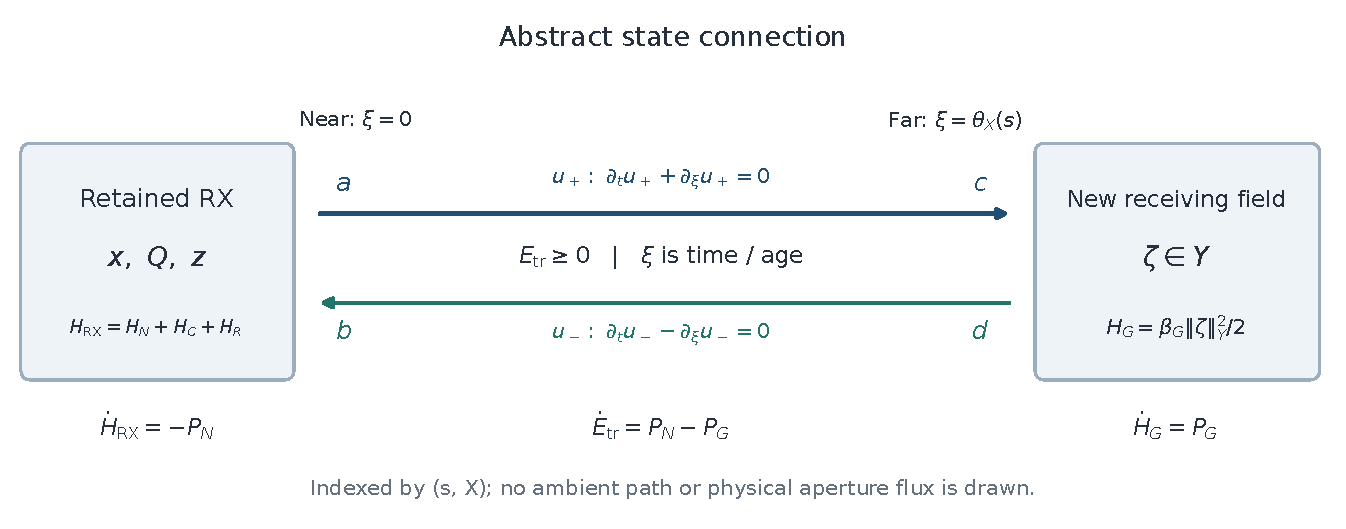
\includegraphics[width=\textwidth]{figures/channel_account.pdf}
\caption{Abstract state connection for a representative channel label $(s,X)$. The near and far powers are sums over the product measure, not physical aperture fluxes. C mixes carrier labels at each X; the receiving field is not six independent point receivers. The coordinate $\xi$ is time/age, and the diagram specifies no ambient curved route.}\label{fig:channel}
\end{figure}

\section{Global forward evolution and augmented conservation}\label{sec:evolution}
The component algebra does not by itself prove a solution theorem. Here the strictly positive minimum delay makes the incoming signals known on each sufficiently short time slab. A local input-energy estimate then continues that slab before total conservation is invoked.

\subsection{Standing assumptions and the solution class}
Fix one admitted positive-width static geometry and hand, finite L,M, positive finite delay bounds $\theta_-,\theta_+$, the retained finite-width H1 profiles, and fixed finite allowed RX coefficients. Let $\kappa\ge0$, $\beta_G>0$. The full state space is
\begin{equation}\label{eq:fullspace}
\mathcal E=\R^6\times U\times\R^2\times\Wcal\times Y.
\end{equation}
The weighted squared norm $2H_{\rm total}$ is equivalent to its product norm at these fixed positive weights. A mild solution means the retained native/old-receiver equations and carrier Duhamel formula, the Hilbert-space receiving ODE, and the characteristic transport formulas, with boundary laws in locally L2 time spaces.

\begin{theorem}[Forward energy-space dynamics]\label{thm:global}
Every finite-energy initial state in $\mathcal E$ has a unique global forward mild solution of~\eqref{eq:closedmodel} with the retained x,z equations and~\eqref{eq:transportPDE}. The full energy state is continuous, x and old z are C1 during exchange, $\zeta$ is locally absolutely continuous, and a,b,c,d are locally L2 in time with values in V. For every exchange-only interval,
\begin{equation}\label{eq:conservation}
\boxed{H_{\rm total}(T)=H_{\rm total}(0),}
\end{equation}
with integrated component identities $\dot H_{\rm RX}=-P_N$, $\dot H_G=P_G$ and~\eqref{eq:linebalance}. The solution depends continuously, in fact locally Lipschitzly on bounded energy sets over each finite horizon, on its initial state in $\mathcal E$.
\end{theorem}

\subsection{Construction before conservation}
\begin{proof}
\textit{Known incoming traces.}
Choose $0<h\le\theta_-$. On $[0,h]$, formulas~\eqref{eq:cstartup}--\eqref{eq:bstartup} give b,c from initial profiles alone up to null endpoints. On $[nh,(n+1)h]$, every delayed boundary argument satisfies $t-\theta_X(s)\le nh$. Thus the incoming b,c are determined by initial profiles or already constructed a,d. The trace estimates~\eqref{eq:tracebounds}, also restricted to subintervals, make them L2 on the current slab. Equality at a slab endpoint changes no L2 class. There is no simultaneous algebraic loop to solve for a current outflow.

\textit{Local forced subsystem.}
Write $X=(x,Q,z)$, and let $\mathcal S(t)=\operatorname{diag}(I,S_c(t),I)$ on the original RX energy space. The source bounds
\begin{equation}\label{eq:localLipschitz}
|f(x)|\le\tfrac12\norm K|x|^2,\qquad
\norm{J_f(x)}\le\norm K|x|,\qquad
|\Bcal^*p|\le\norm\Bcal\norm p_2
\end{equation}
show that the retained polynomial vector field, together with the bounded damping $-\kappa^2Q$, is bounded and locally Lipschitz on every bounded product ball~\cite{RXwellposed}. Denote it by $N_\kappa$. On a slab starting at r, with known b, seek
\begin{equation}\label{eq:newduhamel}
X(t)=\mathcal S(t-r)X(r)+\int_r^t\mathcal S(t-v)
\left[N_\kappa(X(v))+(0,\sqrt2\kappa J^*b(v),0)\right]\dd v.
\end{equation}
The added input is L2 and hence L1 on the finite slab. Its integral can be made small on a short subinterval. On a closed ball in continuous product-space paths, choose that length so the bounded nonlinear term remains in the ball and its local Lipschitz constant times the length is less than one. The integral map is then a contraction. This proves a unique local mild solution without a conservation assumption.

Independently, $-CC^*/\beta_G$ is a bounded nonpositive self-adjoint operator. Its exponential is a contraction. The known c gives
\begin{equation}\label{eq:zetaVOC}
\zeta(t)=e^{-(t-r)CC^*/\beta_G}\zeta(r)
+\frac{\sqrt2}{\beta_G}\int_r^t e^{-(t-v)CC^*/\beta_G}Cc(v)\dd v.
\end{equation}
This unique receiving solution is continuous and absolutely continuous, indeed H1 in time on each finite slab. Its finiteness follows directly from the bounded generator and L1 input.

\textit{Legitimate work for an L2 carrier.}
For the local carrier put $v(t)=S_c(-(t-r))Q(t)$. Duhamel's formula makes this interaction variable absolutely continuous in U, with a.e. derivative
\begin{equation}\label{eq:interactionderivative}
\dot v(t)=S_c(-(t-r))\left[(\Bcal q(t),0)-\kappa^2Q(t)+\sqrt2\kappa J^*b(t)\right].
\end{equation}
The Hilbert norm chain rule and unitarity compute the derivative of $\norm Q^2=\norm v^2$ by pairing Q with the bracket. No differentiation of the unbounded $A_cQ$ is required for L2 preparation. The finite-dimensional right sides depend continuously on x,Q,z through bounded ports, so x,z are C1 and satisfy their usual chain rules. The original reciprocal cancellation and~\eqref{eq:componentpowers} now give the local identity and inequality
\begin{equation}\label{eq:slabenergy}
H_{\rm RX}(t)-H_{\rm RX}(r)
=\frac12\int_r^t\left(\norm{b(v)}_V^2-\norm{a(v)}_V^2\right)\dd v
\le\frac12\int_r^t\norm{b(v)}_V^2\dd v.
\end{equation}

\textit{Continuation on the slab.}
The right side is already known and finite, and $H_{\rm RX}$ controls every component of X. Hence a local solution cannot become unbounded before the slab endpoint. More explicitly, on the resulting bounded ball $N_\kappa(X)$ is bounded and the known forcing is L1. The full interaction variable $\mathcal S(-(t-r))X(t)$ has an integrable derivative, so it has a limit at a putative finite maximal endpoint. Strong continuity of the group gives a limit for X. Restarting the local integral construction there contradicts maximality. This continues X through the slab without presupposing total conservation or carrier H1 regularity.

\textit{Transport and the global account.}
The outgoing laws make $a=\sqrt2\kappa JQ-b$ and $d=\sqrt2C^*\zeta-c$ L2 on the slab. Lemma~\ref{lem:transport} constructs a continuous transport state and proves its integrated work. The receiving norm chain rule in~\eqref{eq:zetaVOC} gives $\dot H_G=P_G$ a.e. Adding these established component identities to~\eqref{eq:slabenergy} proves~\eqref{eq:conservation}. The next slab has known incoming traces, so induction covers every finite forward horizon. Adjacent states join continuously; x,z right sides also join continuously. $\zeta$ is locally absolutely continuous across the finitely many slab joins on any finite horizon. General boundary signals remain only L2 in time.

\textit{Uniqueness and dependence.}
Identical preparations give identical first incoming traces and unique forced subsystem solutions; the outgoing histories and characteristic states then agree. Induction proves uniqueness. For two preparations in a common bounded energy ball, the proved conservation keeps both states in a common bounded ball. Duhamel and a scalar integral inequality on a slab yield
\begin{align}
\norm{\Delta X}_{C([r,r+h])}&\le K_h\left[\norm{\Delta X(r)}+\sqrt h\norm{\Delta b}_{L^2([r,r+h];V)}\right],\notag\\
\norm{\Delta\zeta}_{C([r,r+h];Y)}&\le\norm{\Delta\zeta(r)}_Y
+\frac{\sqrt{2h}\norm C}{\beta_G}\norm{\Delta c}_{L^2([r,r+h];V)}.\label{eq:dependence}
\end{align}
The outgoing differences are bounded by these suprema and the incoming L2 differences. Equation~\eqref{eq:tracebounds} bounds incoming differences by initial-profile differences and previous outgoing-history differences. The characteristic energy identity for differences also gives
\begin{equation}\label{eq:lineDifference}
\sup_{t\le H}\norm{\Delta(u_+,u_-)(t)}_{\Wcal}^2
\le\norm{\Delta(u_{+,0},u_{-,0})}_{\Wcal}^2
+\int_0^H(\norm{\Delta a}_V^2+\norm{\Delta d}_V^2)\dd t.
\end{equation}
Only finitely many slabs occur for fixed H and positive $\theta_-$. Induction gives a finite Lipschitz bound for the continuous energy state and boundary L2 histories in terms of the initial energy-space difference. Its constants depend on the energy bound, fixed parameters and horizon, as asserted.
\end{proof}

The theorem makes no global H1 or backward-flow assertion and no estimate uniform in a zero-delay limit or over unbounded parameter families. Arbitrary L2 initial profiles need no classical boundary-corner compatibility. The energy bound controls states, not instantaneous traces. These restrictions are essential distinctions from the temporary H1 argument used later for one chosen activity preparation.

\begin{remark}[Receiving is reversible]\label{rem:nonmonotone}
The new receiving stock need not be monotone. With empty lines and $C^*\zeta_0\ne0$, c is zero initially. The bounded receiving ODE gives
$H_G'(0+)=-\norm{C^*\zeta_0}_V^2<0$.
The released stock enters the backward-traveling field, consistently with total conservation. This is not irreversible disposal.
\end{remark}

\section{C6 under loading, preparation and native stepping}\label{sec:preparation}
The stateful model earns its account from the component dynamics. It does not remove the temporal-adjoint result of Section~\ref{sec:observation}. We now identify precisely the retained observation and the effect of preparing independent line states.

\subsection{Initial-value and compatible-history formulas}
For nonnegative-time histories define
\begin{equation}\label{eq:delayplus}
(D_\theta^+h)(s,X,t)=\ii_{t\ge\theta_X(s)}h(s,X,t-\theta_X(s)),\qquad
c_{\rm init}(s,X,t)=\ii_{0\le t<\theta_X(s)}u_{+,0}(s,X,\theta_X(s)-t).
\end{equation}
The startup term is L2 in time by Lemma~\ref{lem:transport}. Substituting the actual near boundary law into~\eqref{eq:cstartup} gives
$c=\sqrt2\kappa D_\theta^+JQ-D_\theta^+b+c_{\rm init}$.
Applying C and the receiving ODE proves the exact identity
\begin{equation}\label{eq:loadedC6}
\boxed{\begin{aligned}
\beta_G\dot\zeta&=2\kappa\KGz Q-\sqrt2CD_\theta^+b
+\sqrt2C c_{\rm init}-CC^*\zeta,\\
\KGz&=CD_\theta^+J.
\end{aligned}}
\end{equation}
This holds in locally L2 time with values in Y for every finite-energy preparation. The startup contribution has a plus sign, and the two $\sqrt2$ factors produce the direct coefficient $2\kappa$. Here $\KGz$ is C6 with a specified zero extension of Q as an algebraic decomposition. That extension does not infer that an arbitrary physical past was zero. Independent forward profiles carry separate preparation and need not coincide with a past RX trajectory.

\begin{proposition}[Compatible complete histories]\label{prop:completehistory}
Suppose the required negative-time histories are supplied, with
\begin{equation}\label{eq:historycompatibility}
u_{+,0}(s,X,\xi)=a(s,X,-\xi),\qquad
a+b=\sqrt2\kappa JQ
\end{equation}
on those times as well as forward in time. Then
\begin{equation}\label{eq:completeC6}
\boxed{\beta_G\dot\zeta=2\kappa\KG Q-\sqrt2CD_\theta b-CC^*\zeta.}
\end{equation}
\end{proposition}
\begin{proof}
For $t<\theta$, the compatible startup expression is $a(s,X,t-\theta)$; for $t\ge\theta$, the same expression comes from the boundary. Thus $c=D_\theta a$. Substitute the negative-time and forward near law and use~\eqref{eq:factorization}. Suitable L2 histories on the needed finite interval justify each term by time translation.
\end{proof}

A Q history alone does not imply~\eqref{eq:historycompatibility}, which also involves a and b. Supplied histories satisfying an identity are not automatically histories generated by the full new model; no backward-existence theorem has been used. After $t\ge\theta_+$ the startup term in~\eqref{eq:loadedC6} vanishes a.e. and all its delayed arguments are nonnegative.

Both formulas are causal. Their $C^*$ is a same-time spatial adjoint, not the finite-window temporal $\KG^*$. C6 remains an exact direct component of the actual Q history, but neither $\zeta$ nor its full loaded drive is generally bare C6. Return and loading, and for arbitrary preparation startup, remain explicit. Nonnegative $E_{\rm tr}(0)$ is a quadratic stock of new states; it is not the signed bilinear $W_{\rm pre}$ of~\eqref{eq:testpre} under a new name.

\subsection{The unchanged native map and finite hybrid}\label{sec:native}
Retain the exact original tuple~\cite{RXhybrid}
\begin{equation}\label{eq:nativetuple}
\epsilon=\frac1{10},\quad g=\frac1{60},\quad \lambda_N=\frac1{300},\quad
k=\left(\frac{999}{1000},1,\frac{1001}{1000}\right).
\end{equation}
For $\Omega\in\CC^3$, all components use the same original state for the simultaneous prestage and the same prestage for synchronization:
\begin{align}
\widetilde\Omega_i&=\Omega_i+\epsilon(k_i-|\Omega_i|^2)\Omega_i
+g\sum_{j\ne i}(\Omega_j-\Omega_i),\label{eq:prestage}\\
\delta_i&=\lambda_N\sum_{j\ne i}\sin\!\left(3[\operatorname{Arg}_0\widetilde\Omega_j-\operatorname{Arg}_0\widetilde\Omega_i]\right),
&\Fn(\Omega)_i&=e^{i\delta_i}\widetilde\Omega_i.\label{eq:nativemap}
\end{align}
The convention is $\operatorname{Arg}_0(0)=0$; exact zero prestage components remain zero after rotation. No normalization, coefficient change or continuous-gradient substitute is made.

At a native jump apply this map only to x and leave Q,z,$u_+,u_-,\zeta$ unchanged. Then perform the new exchange stage for a fixed symbolic positive dwell. This is F-first/exchange-second, not a numerical integration scheme.

\begin{proposition}[Finite native-step account]\label{prop:hybrid}
Every finite native/exchange iterate is defined for finite initial energy. For a finite window with post-jump endpoint values,
\begin{equation}\label{eq:hybridbalance}
\boxed{H_{\rm total}(t_b)-H_{\rm total}(t_a)
=\sum_{t_a<t_j\le t_b}\frac{\alpha_N}{2}
\left[I(\Fn\Omega(t_j^-))-I(\Omega(t_j^-))\right]=B_N.}
\end{equation}
\end{proposition}
\begin{proof}
Only native storage changes at each jump; its increment is the summand. Exchange conserves total stock by Theorem~\ref{thm:global}. Summation with the source endpoint convention proves~\eqref{eq:hybridbalance}. A jump at the left endpoint is already in its post-jump value, while one at the right is counted. Finite native inputs have finite polynomial prestages and defined finite images under the zero convention. The global exchange theorem supplies the next interval. Induction gives every finite iterate, without a uniform infinite-step bound.
\end{proof}

The baseline increment is not additional port work or automatically a specified external physical source. No extra impulses are introduced. Nor does finite existence imply continuity across singular native prestages, preservation of a coherent domain, an increasing-step-count limit or recovery after repeated preloaded native updates. Those qualifications remain as in the accepted cadence work~\cite{CAD}.

\subsection{True zero-coupling recovery and D01}
At $\kappa=0$, $\FF=0$ for every incoming b, so the original RX subsystem is recovered for \emph{every} added-state preparation. The isolated new subsystem has $a=-b$, hence $P_N=0$, and can evolve using its own conserved $E_{\rm tr}+H_G$. Empty added states stay empty by uniqueness.

\begin{remark}[Stationary nonempty preparation; D01]\label{rem:D01}
Empty added states are sufficient, not necessary, for inactivity at zero coupling. Choose nonzero $h\in L^2(G)$ and a unit normal n to the carrier plane, and prepare
\begin{equation}\label{eq:inactivekernel}
\kappa=0,\qquad u_{+,0}=u_{-,0}=0,\qquad \zeta_0(X)=(0,h(X)n)\ne0.
\end{equation}
Since $C^*\zeta_0=CC^*\zeta_0=0$, all boundary waves remain zero and $\zeta(t)=\zeta_0$ has positive constant stock. The old RX preparation can be arbitrary and decoupled. This is D01's correction to an earlier work-order necessity sentence; the candidate equations and analytical theorem are unchanged~\cite{Treview}.
\end{remark}

At positive coupling the force changes Q and hence the coupled trajectory. Keeping the native and old-z equations in the same algebraic form does not automatically transfer their earlier capacity, credit, convergence or receiving/recovery theorems. Their actual hypotheses and invariants must be checked again for such a use.

\section{Empty-state latency and a carrier-funded activity witness}\label{sec:activity}
Finite energy and a matched work account permit activity, but neither forces it for every preparation. This section first proves a latency bound for arbitrary RX preparation with empty added states. It then chooses one preparation for which both strict receiving and a later nonzero incoming return can be proved. The two conclusions concern different quantities.

\subsection{What emptiness delays}
\begin{proposition}[Latency]\label{prop:latency}
If $u_{+,0}=u_{-,0}=0$ and $\zeta_0=0$, then for arbitrary finite-energy RX preparation,
\begin{equation}\label{eq:latency}
H_G(t)=0\quad(0\le t\le\theta_-),\qquad
b(t)=0\quad\textnormal{a.e. on }[0,2\theta_-).
\end{equation}
\end{proposition}
\begin{proof}
Before $\theta_-$, the forward characteristic has not crossed any interval. Its initial-profile part is zero, so c is zero a.e. The receiving variation-of-constants formula with zero initial data gives $\zeta=0$, hence d is zero there. Before $2\theta_-$, b is either its zero initial-profile part or d at $t-\theta_X(s)<\theta_-$; this is again zero. Continuity of $\zeta$ includes the endpoint $t=\theta_-$ in the stock statement. No instantaneous trace value at either onset is needed.
\end{proof}
Thus the incoming force $\sqrt2\kappa J^*b$ is delayed, while the term $-\kappa^2Q$ acts immediately to launch the forward field. The result does not say that either stock or boundary trace must become nonzero at its threshold.

\subsection{A preparation with strict receiving}
Fix $\kappa>0$ and prepare
\begin{equation}\label{eq:preload}
x_0=0,\quad z_0=0,\quad Q_0(s)=(P,0),\quad P>0,\qquad
u_{+,0}=u_{-,0}=0,\quad\zeta_0=0.
\end{equation}
Since $f(0)=J_f(0)=0$, uniqueness keeps x identically zero during exchange. Old z continues to obey its retained equation; it is not clamped to zero. Before $2\theta_-$ there is no incoming b, and the carrier satisfies
\begin{equation}\label{eq:earlycarrier}
Q(t)=e^{-\kappa^2t}S_c(t)Q_0+
\int_0^t e^{-\kappa^2(t-v)}S_c(t-v)(\Bcal q(v),0)\dd v.
\end{equation}
The finite-width profiles are H1 and q is continuous, so the integral is continuous into $H^1_{\rm per}$ on every closed interval before $2\theta_-$. The one-dimensional periodic embedding $H^1\hookrightarrow C^0$ and continuity at the constant initial state give some $0<\varepsilon<\theta_-$ such that
\begin{equation}\label{eq:earlypositive}
p(s,u)>P/2,\qquad |Q(s,u)|\le2P
\quad(s\in S_L,\ 0\le u\le\varepsilon).
\end{equation}
This temporary regularity follows from this preparation and equation, not from the energy bound alone. Zero initial line profiles and a nonzero boundary launch at zero are permitted in the mild solution class; no corner compatibility or later global H1 claim is introduced.

\begin{proposition}[Strict receiving from carrier preload]\label{prop:receiving}
For~\eqref{eq:preload} and sufficiently small $\varepsilon>0$ as above,
\begin{equation}\label{eq:strictreceiving}
0<H_G(t)\le LP^2/2\qquad
(\theta_-<t<\theta_-+\varepsilon).
\end{equation}
\end{proposition}
\begin{proof}
Every arrival in this interval samples a near time in $[0,\varepsilon)$, where b is zero. Hence $c=\sqrt2\kappa\ii_{t\ge\theta}JQ(t-\theta)$. The scalar block of the Gram matrix decouples from the vector block and gives
\begin{equation}\label{eq:scalarreceiving}
\beta_G\partial_t\zeta_{\rm sc}(X,t)+m_0(X)\zeta_{\rm sc}(X,t)
=2\kappa a_o\int_{\theta_X(s)\le t}\frac{p(s,t-\theta_X(s))}{d_X(s)}\dd s\ge0.
\end{equation}
Its integrating-factor formula, starting from zero, proves nonnegativity. For strict positivity at any fixed $t\in(\theta_-,\theta_-+\varepsilon)$, choose $\theta_-<r<t$. A minimizing pair for the continuous delay exists on the compact labeled geometry. A relative product neighborhood has $\theta<r$. If its G point is a tip or elbow, move into an adjacent segment interior while preserving the strict inequality. Shrink to a circle interval I and an interior G interval J of positive arclength with $\sup_{I\times J}\theta<r$.

For $X\in J$ and $v\in[r,t]$, the I contribution to the right side of~\eqref{eq:scalarreceiving} is at least $\kappa a_oP|I|/(c_e\theta_+)$. Consequently
\begin{equation}\label{eq:strictlower}
\zeta_{\rm sc}(X,t)\ge
\frac{\kappa a_oP|I|}{\beta_Gc_e\theta_+}
\int_r^t e^{-m_0(X)(t-v)/\beta_G}\dd v>0
\quad\textnormal{for a.e. }X\in J.
\end{equation}
Positive arclength of J gives $H_G(t)>0$. This argument works for every t strictly above the minimum; it requires neither delay differentiation nor an interior minimizer. Since $\zeta$ is continuous in Y, the all-times stock assertion is meaningful. Conservation bounds it by the initial total stock $LP^2/2$.
\end{proof}
The witness is funded by the declared carrier preload. It establishes no native empty-launch receiving, recovery, capacity fraction, or equal and simultaneous activity at all six labels.

\subsection{A later nonzero incoming return}
\begin{proposition}[Incoming boundary activity]\label{prop:return}
The same preparation admits a further reduction of $\varepsilon$ such that
\begin{equation}\label{eq:returnnonzero}
\norm{b(t)}_V>0\quad\textnormal{for a.e. }t\in(2\theta_-,2\theta_-+\varepsilon).
\end{equation}
\end{proposition}
\begin{proof}
The early formula for c, $|A_sQ|=|Q|$, and~\eqref{eq:earlypositive} give
\begin{equation}\label{eq:earlyCbound}
\norm{Cc(v)}_{L^\infty(G)}\le\frac{2\sqrt2\kappa a_oPL}{\delta_w}
\quad(\theta_-\le v\le\theta_-+\varepsilon).
\end{equation}
The positive semidefinite pointwise matrix $\Gmat(X)$ has a contraction exponential. Its receiving formula therefore supplies a representative with
\begin{equation}\label{eq:earlyzetabound}
\norm{\zeta(v)}_{L^\infty(G)}\le
\frac{4\kappa a_oPL}{\beta_G\delta_w}(v-\theta_-).
\end{equation}
This bound uses the bounded early forcing of this witness; it is not an L-infinity theorem for arbitrary energy preparations. Shrink $\varepsilon$ without losing~\eqref{eq:earlypositive} so that
\begin{equation}\label{eq:epsreturn}
\varepsilon<\frac{\beta_G\delta_w^2}{16a_o^2ML}.
\end{equation}
For $2\theta_-<t<2\theta_-+\varepsilon$ and a channel with $\theta=\theta_X(s)<t/2$, set $v=t-\theta$ and $u=t-2\theta$. Then $\theta_-<v<\theta_-+\varepsilon$ and $0<u<\varepsilon$. Its scalar arrival and far effort obey
\begin{align}
c_p(s,X,v)&=\frac{\sqrt2\kappa}{\sqrt M}p(s,u)>
\frac{\kappa P}{\sqrt{2M}},\notag\\
\abs{\sqrt2(C^*\zeta(v))_p(s,X)}&\le
\frac{4\sqrt2\kappa a_o^2P\sqrt M L}{\beta_G\delta_w^2}\varepsilon
<\frac{\kappa P}{2\sqrt{2M}}.\label{eq:effortbound}
\end{align}
The far law and backward characteristic now yield
\begin{equation}\label{eq:negativeb}
b_p(s,X,t)=d_p(s,X,t-\theta)<-\frac{\kappa P}{2\sqrt{2M}}<0
\quad\textnormal{on }\{\theta_X(s)<t/2\}.
\end{equation}
The same relative-neighborhood argument used in the receiving proof gives this sublevel set positive product measure for every $t>2\theta_-$. Thus the L2 trace is nonzero for a.e. t in the asserted interval. The bounded early carrier and pointwise receiving formulas also define a characteristic representative for which the inequality holds at every such t. The energy-space conclusion needs no particular representative at a single onset time.
\end{proof}
The constant 16 in~\eqref{eq:epsreturn} makes the effort bound strictly less than half the direct lower bound. Nonzero b is distinct from $J^*b\ne0$, positive net carrier work, native credit and recovery. Projection and simultaneous launch still enter the actual force. Figure~\ref{fig:time} separates these latency results from the temporal-adjoint support of Section~\ref{sec:observation}.

\begin{figure}[tbp]\centering
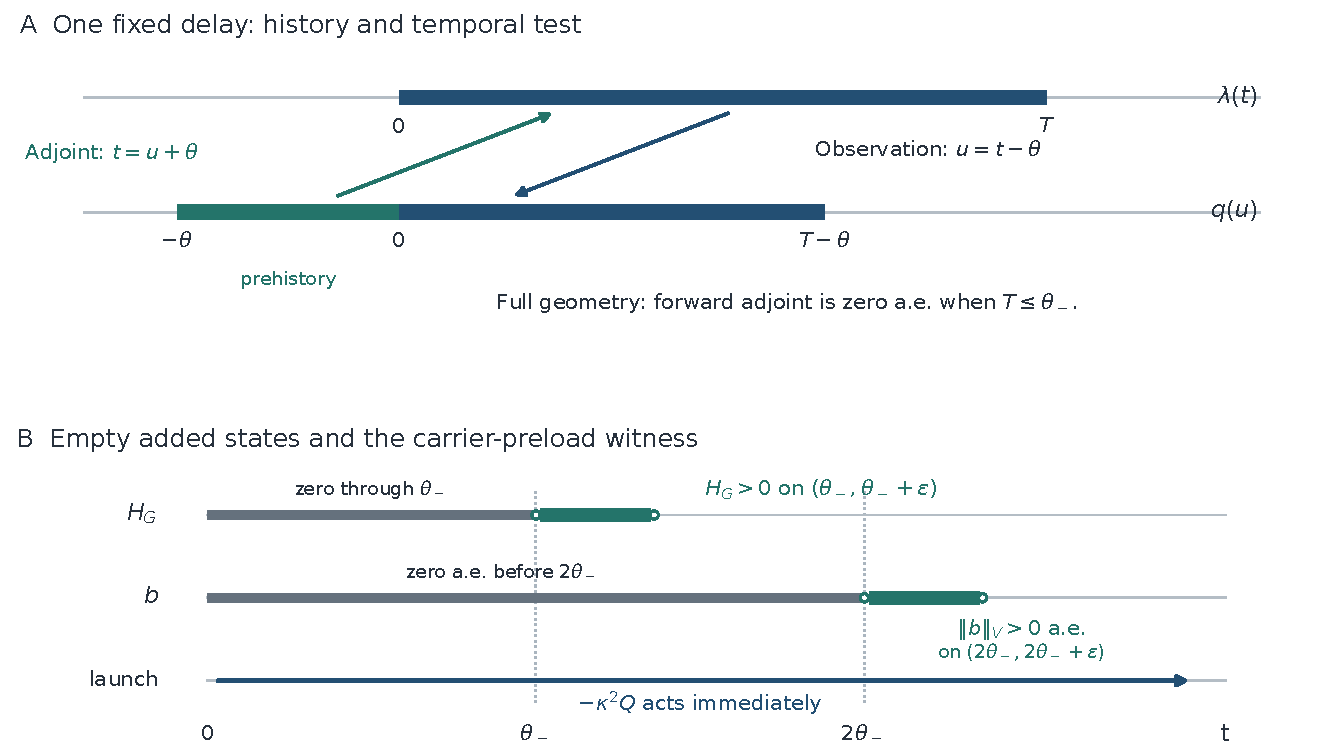
\includegraphics[width=\textwidth]{figures/time_support.pdf}
\caption{Two different time accounts. Top: for one fixed delay, causal observation reads earlier carrier data, while the finite-window temporal adjoint evaluates a later test time and has a prehistory part. Bottom: empty added states impose the proven latency bounds; the constant carrier-preload witness gives strict receiving and a nonzero incoming boundary trace on short open intervals. Interval lengths and positions are schematic. These are supports and bounds, not simulated waveforms or exact onset amplitudes.}\label{fig:time}
\end{figure}

\section{What the connection establishes, and what remains spatial}\label{sec:discussion}
The observation and transport investigations answer complementary questions. A delayed C6 readout is a bounded causal map on the correct history space. Its temporal dual is determined by that domain and the finite test window, not by a physical transmission mechanism. The signed prehistory term identifies the part of the work pairing that cannot be charged to the forward carrier interval. By contrast, the extension declares additional traveling fields and a separate receiving state, and proves their evolution and work account. The new preparation carries a nonnegative quadratic stock. It is not W's signed bilinear prehistory pairing in another notation.

The constructive result is substantial at its stated level: positive stocks, global forward mild evolution, exact total exchange conservation, the full loaded C6 identity, and a receiving/return witness. Its straight endpoint distance enters as static delay data. The coordinate $\xi$ is time or age, and no map from each interval into an ambient curved path has been selected. If a physical rectifiable path connects the two endpoints, its length $\ell$ satisfies $\ell\ge d_X(s)$. A genuine detour at the same constant speed would change its travel time from $d_X(s)/c_e$ to $\ell/c_e$. The current Euclidean delay therefore cannot by itself certify traversal of an outward--around--inward curve.

The author's intended picture includes stationary supports, a central meeting region, opposed directions, outward spreading, curved return, and possible transfer elsewhere. Local exchange and a larger circuit are compatible aims. To attach this candidate to that picture, one must specify the physical locations of its channel and receiving fields, their material or effective energy density, the relation between delay and route length, and the meaning of overlap among channels indexed by $(s,X)$. The product measure $\dd s\dd\ell\dd\xi$ is a declared mathematical metric; it does not already count distinct physical volumes. A physical clock, speed or load interpretation also requires correspondence beyond the units check. This paper makes no new choice of diversion fraction, material receiver or geometric route.

G remains the six actual labeled broken boundaries with arclength measure. It is not a set of filled apertures, and the new receiving equation is not an aperture-flux law. The old carrier, tight toroid, close diagnostic ball, outer arrangements, old z and new $\zeta$ retain their separate meanings. The separation established in the central-route/six-opening investigation remains an inherited fact; this state extension does not silently move the old carrier onto an opening or identify host-notch contacts with central crossings~\cite{centralpaper,SOreview}.

Three qualifications prevent an algebraic account from being interpreted as more than it proves. First, receiving stock can decrease, and a nonzero incoming b does not itself prove positive projected feedback or native credit. The witness has x identically zero. Second, at positive $\kappa$ the carrier trajectory and coupled native history change. Earlier trajectory-dependent capacity, receiving/recovery, credit and convergence conclusions require their hypotheses to be checked anew. The completed exchange-only achievements are not reopened, but neither are their conclusions automatically transferred to the modified trajectories. Third, a physical attribution of phase or arrival time needs the relevant state and preparation information. Common-phase statements remain conditional; instantaneous readouts do not recover arbitrary delay histories.

The earlier Q01 qualification is retained: an inner gap can supply a positive delay to a specified cut, but that cut-dependent statement is not a universal no-delay theorem for all receiver work. The cadence and singular-prestage restrictions also remain those of the accepted native map. Finite iterates in Section~\ref{sec:native} do not remove the map's singular set or give a bound uniform over infinitely many steps. An autonomous native reconstruction result for the old uncoupled history is not a reconstruction theorem for the present coupled evolution~\cite{CAD,RXhybrid}.

The accepted W record contains four scoped exact-algebra groups and the T record five separate groups. They corroborate specified algebra; they are not numerical substitutes for the functional, trace and positive-measure proofs reproduced here. The present preparation preserves those code/log records and acceptance decisions without adding a scientific rerun. Document compilation, source integrity and page inspection are recorded separately from mathematical acceptance.

This completes the mathematical observation and declared transport/storage assessment. A physical embedding and account relating the transport coordinate, product metric and receiving field to the intended route remain open correspondence questions. They are not missing steps in the forward solution theorem established here.

\appendix
\section{Notation and dimensional crosswalk}\label{app:notation}
The two investigations reused several symbols for different objects. The present notation separates those roles; the external claim ledger retains the original source names. No mathematical equation is changed by these editorial renamings.

\begin{longtable}{>{\raggedright\arraybackslash}p{.24\textwidth}>{\raggedright\arraybackslash}p{.69\textwidth}}
\toprule Symbol & Meaning in this manuscript\\\midrule\endhead
$w,\tau_g$ & Common host width and fixed static geometry parameter; $\tau_g$ is not time.\\
$R_{\rm ball},\rho_\perp$ & Diagnostic ball radius and cylindrical radius, respectively.\\
$S_L,L,s$ & Periodic carrier, its length and its arclength coordinate.\\
$G,M,X,\ell$ & Labeled union of six actual broken arcs, total arclength, point and arc measure coordinate.\\
$d_X(s),\delta_w$ & Endpoint distance and inherited positive clearance lower bound.\\
$\theta_X(s),\theta_-,\theta_+,\Theta$ & Actual delay, its minimum and maximum, and sufficient history horizon.\\
$A^\perp_{\tau_g},J_\perp$ & Horizontal geometric map and planar quarter-turn.\\
$Q=(p,r_c),U$ & Carrier field and its real L2 space.\\
$\Bcal,q,z,\beta_R$ & Old finite-profile source map, two-component port, old receiving state and its metric.\\
$A_s,Y$ & Scalar/tangent-vector inclusion and receiving-field L2 space.\\
$U_o,V_o$ & Scalar and vector C6 readouts; not Hilbert-space names.\\
$\KG,\KGz,\KG^*$ & Complete-history observation, zero-prehistory restriction and temporal adjoint.\\
$J,V,C,C^*$ & Normalized replication, product channel space, spatial mixing and same-time spatial adjoint.\\
$\Gmat(X),m_0(X)$ & Spatial Gram matrix and its scalar block; the T source calls the matrix B.\\
$\xi,\Wcal,u_+,u_-$ & Time/age coordinate, transport space and its two traveling fields.\\
$a,b,c,d$ & Near forward outflow, near incoming return, far arrival and far return outflow.\\
$\zeta,\beta_G,H_G$ & New receiving field, its positive metric coefficient and its stock.\\
$H_{\rm RX},E_{\rm tr},H_{\rm total}$ & Retained RX, transport and total augmented stocks.\\
$P_N,P_G,B_N$ & Near power, far receiving power and finite native-map baseline increment.\\
\bottomrule
\end{longtable}

For a dimensional check let $[s]=[\ell]=\mathsf L$, $[\xi]=[t]=\mathsf T$, $[Q]=\mathsf U$ and $[g_o]=\mathsf G_o$, so $a_o=g_o/(4\pi)$. A compatible dimensional assignment for the declared extension is
\begin{align}
[\kappa]&=\mathsf T^{-1/2},&
[a]=[b]=[c]=[d]&=\mathsf U\mathsf L^{-1/2}\mathsf T^{-1/2},\notag\\
[\zeta]&=\mathsf U\mathsf G_o^{-1}\mathsf T^{-1/2},&
[\beta_G]&=\mathsf G_o^2\mathsf T,\notag\\
[Cc]&=\mathsf U\mathsf G_o\mathsf T^{-1/2},&
[\FF]&=\mathsf U\mathsf T^{-1},\label{eq:units}\\
[H_{\rm RX}]=[E_{\rm tr}]=[H_G]&=\mathsf U^2\mathsf L,&
[P_N]=[P_G]&=\mathsf U^2\mathsf L\mathsf T^{-1}.\notag
\end{align}
The old metric remains $[\beta_R]=\mathsf T^2/\mathsf L$. In particular $[\beta_G]\ne[\beta_R]$ in general. Integrating transport density over $\dd s\dd\ell\dd\xi$ gives the same stock dimension as the carrier. These are consistent declared units, not a derivation of material energy density or a calibration of a physical clock.

\section{A scalar illustration of signed prehistory}\label{app:example}
To make the sign in~\eqref{eq:prehistorybalance} transparent, consider only the scalar delay map $y(t)=q(t-2)$ with $q(u)=u+3$, test $\lambda(t)=t+1$ and window $[0,T]$. This is an algebraic illustration from the accepted W record, not an RX trajectory or a simulation. Define
\begin{align*}
W_{\rm test}&=\int_0^Tq(t-2)\lambda(t)\dd t,\\
W_{\rm pre}&=\int_{-2}^0q(u)\widetilde\lambda(u+2)\dd u,\\
J_{\rm fwd}&=\int_0^Tq(u)\widetilde\lambda(u+2)\dd u,
\end{align*}
where the test is zero outside $[0,T]$. A change of variable gives $W_{\rm test}=W_{\rm pre}+J_{\rm fwd}$. Direct integration gives
\begin{center}\begin{tabular}{cccc}\toprule
$T$ & $W_{\rm test}$ & $W_{\rm pre}$ & $J_{\rm fwd}$\\\midrule
1 & $7/3$ & $7/3$ & 0\\
2 & $26/3$ & $26/3$ & 0\\
3 & 21 & $26/3$ & $37/3$\\\bottomrule
\end{tabular}\end{center}
The short windows have no forward dual work. If a conditional negative-adjoint force supplies $\Delta H_{\rm RX}-B_N=-J_{\rm fwd}$, its balance is precisely $\Delta H_{\rm RX}+W_{\rm test}-B_N=W_{\rm pre}$, with a positive coefficient on the signed prehistory pairing. Replacing $\lambda$ by $-\lambda$ reverses the sign. Nonzero prehistory need not give nonzero work: with $q(u)=u+1$, $\lambda=1$ on $[0,3]$, the prehistory integral is $\int_{-2}^0(u+1)\dd u=0$. No positive stored energy is defined by that bilinear term.

\section{Accepted-claim coverage and reproducibility}\label{app:coverage}
The manuscript integrates the two accepted project-internal records~\cite{Wreview,Treview}. Its mathematical scope is unchanged. The following map gives the principal locations; the delivered machine-readable ledger additionally records all supporting equation labels, resolved numbers/pages, exact source-line spans, hypotheses, limits and SHA-256 identities.

\begin{longtable}{>{\raggedright\arraybackslash}p{.10\textwidth}>{\raggedright\arraybackslash}p{.41\textwidth}>{\raggedright\arraybackslash}p{.41\textwidth}}
\toprule Record & Accepted content & Principal manuscript location\\\midrule\endhead
W01 & Static geometry, clearance, history horizon & Proposition~\ref{prop:geometry}; \eqref{eq:clearance}--\eqref{eq:ballmargin}\\
W02 & Complete-history observation and boundedness & Theorem~\ref{thm:observation}; \eqref{eq:pointunbounded}\\
W03 & Temporal adjoint and advanced dependence & Proposition~\ref{prop:adjoint}; \eqref{eq:futureepsilon}\\
W04 & Present carrier does not specify arbitrary history & Proposition~\ref{prop:presenthistory}\\
W05 & Conditional work, native increments and signed prehistory & Proposition~\ref{prop:conditionalwork}, Corollary~\ref{cor:prehistory}\\
T01 & Spatial factorization and Gram/kernel structure & Proposition~\ref{prop:factorization}\\
T02 & L2 transport, traces and integrated work & Lemma~\ref{lem:transport}\\
T03 & Declared effort/flow coupling and stocks & \eqref{eq:closedmodel}--\eqref{eq:componentpowers}\\
T04 & Global forward mild evolution and conservation & Theorem~\ref{thm:global}\\
T05 & Loaded direct C6 and compatible complete history & \eqref{eq:loadedC6}; Proposition~\ref{prop:completehistory}\\
T06 & Native-map finite-step account & Proposition~\ref{prop:hybrid}\\
T07 & Latency, strict receiving and incoming return & Propositions~\ref{prop:latency}--\ref{prop:return}\\
D01 & Empty added preparation sufficient, not necessary & Remark~\ref{rem:D01}\\\bottomrule
\end{longtable}

The edition contains all TeX content and both deterministic vector figures needed to build the PDF. The build helper uses cached Tectonic in untrusted mode with intermediates outside the edition. Figure source, environment records, build receipts, extracted text, document checks and individual final-page renders are delivered with the review archive. The final-page inspection is bound to the exact PDF digest. Document checks establish artifact fidelity; mathematical acceptance, internal manuscript review and the repository publication receipt remain distinct records.

The source ledger distinguishes preserved equations and accepted proofs from layout/build precedents. Original acceptance archives and current readable dispositions are retained unchanged. W's four exact-algebra groups and T's five are preserved as separate historical corroboration, not described as new tests of this edition. The external wave-variable citation below supplies methodological context from the publisher's indexed abstract and metadata; no unread external theorem is invoked in place of the explicit proofs.

\clearpage
\addcontentsline{toc}{section}{References}
\begin{thebibliography}{99}
\raggedright
\bibitem{niemeyer} G. Niemeyer and J.-J. E. Slotine.
Stable adaptive teleoperation. \emph{IEEE Journal of Oceanic Engineering}
16(1), 152--162 (1991). \href{https://doi.org/10.1109/48.64895}{doi:10.1109/48.64895}.
Methodological context from the publisher's indexed abstract and bibliographic record.

\bibitem{Wreview} Project-internal research record.
\emph{Native Spatial Work Registration 01}: independent proof review, W01--W05,
and GPT acceptance. Accepted research, 2026; not a published edition of this manuscript.
Preserved readable proof, decision and complete acceptance archive in the accompanying package,
under \sourcepath{inputs/accepted/spatial_work/} and \sourcepath{inputs/evidence/spatial_work/}.

\bibitem{Treview} Project-internal research record.
\emph{Native Causal Transport Storage 01}: independent proof review, T01--T07,
and GPT acceptance with D01, 10 November 2026.
Accepted research, not a published edition of this manuscript.
Preserved under \sourcepath{inputs/accepted/causal_transport/} and
\sourcepath{inputs/evidence/causal_transport/}.

\bibitem{centralpaper} H. F. Halldórsson (pzychozen).
\emph{Central-Route Accounting and Six-Opening Geometry in the Reciprocal Chiral Exchange Candidate}.
Research edition v0.1 (2026).
\href{https://github.com/pzychozen/trioctagon-physics/tree/9f02de9335232da9c1732b4851199098d363198b/papers/CENTRAL_ROUTE_SIX_OPENING_CORRESPONDENCE/publication/v0.1}{Immutable repository snapshot, commit 9f02de9}.
Inherited published foundation; no new publication audit is asserted here.

\bibitem{SOreview} Project-internal research record.
\emph{Native Six-Opening Transport Correspondence 01}: accepted proof and GPT disposition (2026).
Preserved under \sourcepath{inputs/accepted/six_opening/}; source identities and the
separation/convex-enclosure scope are retained in the review package.

\bibitem{CAD} Project-internal research record.
\emph{Native F-Stepping Exchange Cadence 01}: accepted proof, cadence status and limits (2026).
Preserved under \sourcepath{inputs/accepted/cadence/}.

\bibitem{CCgeometry} H. F. Halldórsson (pzychozen).
Static centered geometry and actual broken arcs. Retained primary source, \sourcepath{sources/CC/geometry.tex}.
\href{https://github.com/pzychozen/trioctagon-physics/blob/c3ee366bd6195bd7fa77efd0321214af4c2dc173/papers/NATIVE_INTENSITY_AND_CONDITIONAL_CARRIER_CROSSINGS/publication/v0.1/manuscript/geometry.tex}{Immutable source, commit c3ee366}.
Exact preserved bytes and original provenance are recorded in the source ledger.

\bibitem{CCcarrier} H. F. Halldórsson (pzychozen).
Carrier equations and C6 observation. Retained primary source, \sourcepath{sources/CC/carrier.tex}.
\href{https://github.com/pzychozen/trioctagon-physics/blob/c3ee366bd6195bd7fa77efd0321214af4c2dc173/papers/NATIVE_INTENSITY_AND_CONDITIONAL_CARRIER_CROSSINGS/publication/v0.1/manuscript/carrier.tex}{Immutable source, commit c3ee366}.
Exact preserved bytes and original provenance are recorded in the source ledger.

\bibitem{RXcandidate} H. F. Halldórsson (pzychozen).
Reciprocal exchange candidate and profiles. Retained primary source, \sourcepath{sources/RX/candidate.tex}.
\href{https://github.com/pzychozen/trioctagon-physics/blob/6b1ef6494a4d4c34398ba9d9e5a7afce1fb03f37/papers/NATIVE_CAPACITY_RECEIVING_RECOVERY/publication/v0.1/evidence/accepted_investigation/inputs/sources/P1/manuscript/candidate.tex}{Immutable source, commit 6b1ef64}.
Exact preserved bytes and original provenance are recorded in the source ledger.

\bibitem{RXpower} H. F. Halldórsson (pzychozen).
Reciprocal exchange power identities. Retained primary source, \sourcepath{sources/RX/power.tex}.
\href{https://github.com/pzychozen/trioctagon-physics/blob/6b1ef6494a4d4c34398ba9d9e5a7afce1fb03f37/papers/NATIVE_CAPACITY_RECEIVING_RECOVERY/publication/v0.1/evidence/accepted_investigation/inputs/sources/P1/manuscript/power.tex}{Immutable source, commit 6b1ef64}.
Exact preserved bytes and original provenance are recorded in the source ledger.

\bibitem{RXwellposed} H. F. Halldórsson (pzychozen).
Original energy-space well-posedness framework. Retained primary source, \sourcepath{sources/RX/wellposed.tex}.
\href{https://github.com/pzychozen/trioctagon-physics/blob/6b1ef6494a4d4c34398ba9d9e5a7afce1fb03f37/papers/NATIVE_CAPACITY_RECEIVING_RECOVERY/publication/v0.1/evidence/accepted_investigation/inputs/sources/P1/manuscript/wellposed.tex}{Immutable source, commit 6b1ef64}.
Exact preserved bytes and original provenance are recorded in the source ledger.

\bibitem{RXhybrid} H. F. Halldórsson (pzychozen).
Native map and finite hybrid exchange. Retained primary source, \sourcepath{sources/RX/hybrid.tex}.
\href{https://github.com/pzychozen/trioctagon-physics/blob/6b1ef6494a4d4c34398ba9d9e5a7afce1fb03f37/papers/NATIVE_CAPACITY_RECEIVING_RECOVERY/publication/v0.1/evidence/accepted_investigation/inputs/sources/P1/manuscript/hybrid.tex}{Immutable source, commit 6b1ef64}.
Exact preserved bytes and original provenance are recorded in the source ledger.
\end{thebibliography}

\end{document}
